\documentclass[czech,BP]{thesiskiv}

\author{Jan Kohlíček}
\declarationmale

\title{Skladové hospodářství pomocí RFID a Raspberry Pi}

\abstracttexten{The text of the abstract (in English). It contains the English translation of the thesis title and a short description of the thesis.}

\abstracttextcz{Text abstraktu (česky). Obsahuje krátkou anotaci (cca 10 řádek) v češtině. Budete ji potřebovat i při vyplňování údajů o bakalářské práci ve STAGu. Český i anglický abstrakt by měly být na stejné stránce a měly by si obsahem co možná nejvíce odpovídat (samozřejmě není možný doslovný překlad!).
}

\usepackage[nottoc,notlot,notlof]{tocbibind}
\usepackage[pdftex]{graphicx}
\usepackage[pdftex]{hyperref}
\hypersetup{colorlinks=true,
  unicode=true,
  linkcolor=black,
  citecolor=black,
  urlcolor=black,
  bookmarksopen=true}
\usepackage[numbers,sort&compress]{natbib}
\usepackage{color}
\usepackage{xcolor}
\usepackage{multirow}
\usepackage{tabularx}
\usepackage{acronym}
\usepackage{enumitem}
\usepackage{subcaption} 

\begin{document}

\maketitle
\tableofcontents


\chapter{Úvod}
\iffalse
Nástupem čtvrté průmyslové revoluce, označené v České republice jako Průmysl 4.0, se očekává plně automatizovaný proces a 
sdílení informací v tzv. "chytrých továrnách".
Průmysl 4.0 bude využívat informační a kybernetické technologie, datová centra, cloudová úložiště, autonomní roboty a
další. Všechny produkty, zboží i stroje by měly obsahovat čipy, díky kterým je bude možné kontrolovat, obsluhovat, budou 
komunikovat mezi sebou a přes internet i s majitelem či se zákazníkem. 
\\\\
 Cílem této práce je vytvořit serverový systém, takový jeden z prvních kroků "chytrého skladu", který umožní vzdáleně 
komunikovat s klientskou aplikací a samotnou čtečkou RFID. 
Pro systém je nutné vybrat vhodný programovací jazyk a také optimální způsob komunikace mezi klientem a serverem, 
či způsob uložení dat. K tomu mají dopomoci Raspberry Pi 2 a čtečka kódů RFID. 
Součástí práce je vytvořit klientskou část s uživatelským rozhraním pro PC či mobilní zařízení, která umožní 
vizualizaci dat skladového hospodářství. Tato práce také má testovat a analyzovat výhody či nevýhody vybraného řešení.
\\\\
Práce popisuje teoretické řešení skladového hospodářství s využitím čtečky RFID.  
Také se zabývá zefektivněním a zautomatizováním skladového hospodářství. Popisuje různé druhy RFID, jejich výhody a nevýhody.  
\\\\
Dále práce popisuje řešení samotného vývoje skladového systému s využitím RFID.
\\\\
V poslední části se pak zabývám samotným testováním vytvořené aplikace a jejím možným rozšířením a vylepšením. 












1) Seznamte se s Raspberry Pi 2 (RPi), čtečkou čárových (RFID) kódů, zapojením daných zařízení a diskutujte možnosti využití pro skladové hospodářství. Proveďte analýzu problému a zvolte vhodný programovací jazyk. 

2) Vytvořte serverový program, který umožní vzdáleně komunikovat s klientskou aplikací a samotným RFID zařízením.
Vyberte vhodný způsob komunikace mezi klientem a serverem, způsob uložení dat a diskutujte výhody/nevýhody vámi vybraného řešení.

3) Vytvořte klientskou část s uživatelským rozhraním pro PC či mobilní zařízení, která umožní vizualizaci dat skladového hospodářství.

4) Vytvořený systém otestujte, zhodnoťte jeho praktickou použitelnost a diskutujte jeho možná vylepšení.
\fi














	
\chapter{Skladové hospodářství}
Skladové hospodářství je nedílnou součástí logistického systému. Sklady mají za úkol přijímat zásoby, uchovávat a vydávat je a provádět potřebné skladové manipulace. Skladové hospodářství má v podnicích návaznost na téměř všechny ostatní úseky. Hlavním úkolem skladu je ekonomické sladění rozdílně dimenzovaných toků v podniku, a to tak, aby bylo dosaženo synergického efektu.\cite{vitek2007skladove}


\section{Současný skladový systém}
Pod tímto pojmem si můžeme představit systém pro evidenci skladu resp. skladovaných zásob (příjem  a  výdej  materiálu), systém pro účtování zásob a jejich objednávek nebo systém pro inventarizaci. Můžeme tedy říci, že skladový systém je systém pro správu ekonomických operací nad skladem.\cite{hron2014skladovy}


\section{Skladový systém s RFID}

\subsection{Rychlé načtení údajů}
\texttt{RFID} čip má oproti etiketě s čárovým kódem dvě hlavní výhody - rychlost čtení a nepřímou viditelnost čtecího zařízení na čip. Současné standardy \texttt{UHF RFID} čipů umožňují načíst najednou až 1000 čipů za sekundu, tato hodnota se však s příchodem novějších a výkonnějších zařízení bude zvyšovat. \texttt{RFID} čtecí zařízení nepotřebuje mít přímou viditelnost na jednotlivé čipy, čtení i zápis probíhá bezdrátově a to do vzdálenosti cca 15 m u pasivních čipů a až 100 m u aktivních čipů.\cite{dolevcek2010identifikace}
\\
Například paletový přepravník tak může projet celým \texttt{RFID} čtecím portálem a v jeden čas dojde k současnému načtení všech čipů na paletě, tím se dosáhne zrychlení procesu příjmu, výdeje, přesunu a inventarizace produktu.\cite{dolevcek2010identifikace}

\subsection{Odstranění chyb obsluhy}
\texttt{RFID} čipy společně se čtecím zařízením vylučují možnost vzniku chyby obsluhy, které vzniknou například tím, že obsluha načte pouze část \texttt{čárových kódů} na paletě.\cite{dolevcek2010identifikace}

\subsection{Zápis údajů o zboží během celého logistického pohybu}
\texttt{RFID} čip má oproti etiketě s \texttt{čárovým kódem} hlavní výhodu v tom, že do čipu lze informace i zapisovat a nejenom číst, jak je to v případě \texttt{čárového kódu}. Tato vlastnost bude v budoucnosti klíčová a rozhodne v mnoha odvětvích pro úplnou náhradu \texttt{čárového kódu} \texttt{RFID} čipem. Do čipu lze navíc informace zapisovat a měnit opakovaně, lze takto do každého produktu zapsat datum výroby a poté také připsat jednotlivé logistické zápisy, které vznikají po celou dobu cesty produktu.\cite{dolevcek2010identifikace}

\subsection{Přesná evidence spotřebitelských jednotek}
V současnosti při samotném logistickém procesu obsluha načte \texttt{čárový kód} palety, ale již není schopna ověřit, zda je na paletě správný počet kartónů a správný počet produktů. Jediným řešením by bylo paletu rozebrat a postupně načíst všechny \texttt{čárové kódy}. \texttt{RFID} čtecí portál však načte najednou všechny RFID čipy na paletě nalezené. Navíc dle typu čipu dokáže vyhodnotit počet \texttt{RFID} čipů kartónů i počet RFID čipů samotných produktů.\cite{dolevcek2010identifikace}

\subsection{Odolnost RFID čipů}
Etiketa s \texttt{čárovým kódem} podléhá teplotním a povětrnostním vlivům a následně dochází k poškození etikety. Je tomu hlavně proto, že je nutné etikety s \texttt{čárovým kódem} umisťovat tak, aby je bylo možné načíst čtecím zařízením a tudíž zvenku. \texttt{RFID} čip je umístěn uvnitř produktu nebo balení a tím je odolný jak proti teplotě, vodě i povětrnosti. V současné době na trhu již existují \texttt{RFID} čipy, které navíc mohou obsahovat čidla - například pro měření vlhkosti nebo teploty. \cite{dolevcek2010identifikace}


\subsection{Optimalizace skladových zásob}
Představme si tak obvyklou záležitost, jakou je příjem materiálu (zboží) a jeho naskladnění. Tato operace dnes probíhá v mnoha společnostech po jednotlivých kusech (logistických jednotkách), a tak se také informace dostávají do informačního systému (se zpožděním).
Celá došlá zásilka je načtena \texttt{RFID} čtečkami během několika sekund a tato informace (násobně větší objem) se přenáší do informačního systému, který dosud nebyl na tento způsob zpracování informací připraven. Výsledkem tohoto naskladnění je okamžitá informace o stavu našeho skladu, a dramatické zrychlení jejího získání. Vybavíme-li stejnou technologií také výrobu ve společnosti, získáme tak stejné informace z jednotlivých částí výroby (stav výroby, průběžné zásoby na pracovišti). 
Dramatické zrychlení sběru informací v rámci logistiky (výroby) umožňuje daleko lepší plánování zásob společnosti. Pokud máme plán výroby a stavy zásob, tak zásoby, které máme na skladě můžeme odpovědně řídit ne z hlediska \texttt{Q (množství)}, ale z hlediska 
\texttt{T (času)}. Tím se zcela zásadním způsobem zjednodušuje systém predikce objednávek a otevírá se velký prostor pro optimalizaci skladových zásob - úspory na vázaném kapitálu.\cite{dolevcek2010identifikace}



\section{Popis systému RFID-RMS}

Systém \texttt{RFID-RMS} se používá pro poskytovatele logistických služeb ke zlepšení skladových operací pomocí sledování a optimalizace využitých zdrojů. \texttt{RFID-RMS} využívá mobilní technologie k přesnému určení lokalizace, sledování a řízení zdrojů v prostředí skladu. Architektura systému \texttt{RFID-RMS} se skládá ze dvou částí, které přispívají k rozhodovacímu procesu v oblasti řízení zdrojů. První část je \texttt{frontend}, obsahující dva moduly pro sběr dat, a to modul pevných logistických dat a modul proměnných logistických dat. Tyto dva moduly obsahují dva různé typy \texttt{RFID tagů} pro ulehčení přenosu a ukládání logistických dat. Druhá část je \texttt{backend}, který obsahuje modul sledování zdrojů, modul řízení zdrojů a datového úložiště. Primární funkcí této části je provádět řízení zdrojů, sledování zdrojů, hodnotit využití zdrojů, výběr nejvhodnější trasy, údržba a kontrola provozu.\cite{chow2006design}

\subsection{Sběr dat}

\texttt{Modul pevných logistických dat} používá nízkoúrovňové \texttt{radiové} signály pro výměnu dat mezi pasivními \texttt{tagy} a čtečkou. Pasivní \texttt{tag} se skládá z \texttt{integrovaného obvodu} pro uložení identity položek a dalších informací. Jak je znázorněno na obrázku \ref{fig:passive}, pasivní značka je připojena na položky, jako jsou palety, obaly atd. Čtečky tagů s pevnou pozicí antén jsou namontovány do konstrukce jako jsou dveře, vstupní brána nebo integrované do vysokozdvižných vozíků a ostatního vybavení. Obsahuje-li více antén, dokáží v rámci svého rozsahu najednou rozpoznat a číst stovky \texttt{tagů}. Dále budou přijaté signály dekódovány na data a dál poslány pomocí datového připojení k serveru, na kterém běží obchodní logika. Výměna dat mezi čtečkou a řízením zdrojů je zprostředkována prostřednictvím bezdrátové sítě \texttt{LAN}.\cite{chow2006design}
\newpage

\begin{figure}[ht]
		\centering
		\includegraphics[width=0.5\textwidth]{../images/passive.jpg}	
		\caption{Modul proměnných logistických dat\cite{chow2006design}}
		\label{fig:passive}
\end{figure}

K \texttt{modulu proměnných logistických dat} se vztahují ultra-širokopásmové technologie \texttt{(UWB)}, které definují přenos proměnných logistických dat mezi čtečkou a tagem, jak je znázorněno na obrázku \ref{fig:uwb}. Tento modul obsahuje kolekci aktivních tagů, čtyři čtečky \texttt{UWB} a \texttt{Hub procesor} pro sledování polohy zdrojů. \texttt{UWB} aktivní tagy se skládají z interní baterie a krátkého \texttt{impulsového} vysílače umožňujícího vysílat na mnohem delší vzdálenost. \texttt{Tag} vydá krátkodobý \texttt{pulzní} signál několikrát za sekundu. \texttt{UWB} čtečky přijímají signály a posílají je do Hub procesoru. S logickým nastavením\texttt{triangulace} rozdílného čtení \texttt{UWB} čteček lze vypočítat přesné (x, y, z) souřadnice aktivního \texttt{tagu}. Přitom je koordinace zdrojů ve skladu přesně vypočítaná. Takové koordinace zdrojů budou předány \texttt{sledovacímu modulu zdroje} pro následné zpracování.\cite{chow2006design}


\begin{figure}[ht]
		\centering
		\includegraphics[width=0.6\textwidth]{../images/uwb.jpg}	
		\caption{Modul proměnných logistických dat\cite{chow2006design}}
		\label{fig:uwb}
\end{figure}




\subsection{Sledování}
\texttt{Modul sledování zdrojů} je server, který uloží všechny údaje aktivních \texttt{tagů} a poskytuje výkonné prostředí pro manipulaci s daty, filtruje a předává veškeré užitečné údaje řízení zdrojů pro formulování obchodní logiky a rozhodování. To je základem pro řízení zdrojů pro provádění činností včetně řízení zdrojů, plánování zdrojů, využívání a měření výkonnosti. Kromě výše uvedených funkcí, modul sledování je schopný převést data \texttt{UWB} na (x, y, z) souřadnice, které pak poskytují v reálném čase vizuální zobrazení přesného umístění zdroje na mapě skladu.\cite{chow2006design}

\subsection{Řízení}
\texttt{Modul řízení zdrojů} zpracovává data z aktivních \texttt{tagů} v reálném čase. Na základě těchto informací hledá optimální trasu a délku cesty k vyzvednutí zdrojů každým potenciálním manipulačním zařízením. V důsledku toho je vybráno zařízení nejvhodnější pro provedení úkolu.\cite{chow2006design}
	


\chapter{Popis zařízení}
	\section{Raspberry Pi}
		\texttt{Raspberry Pi (RPi)} je řada malých jedno deskových počítačů, vyvíjená ve Velké Británii.\\		
		Pro tento projekt se použije \texttt{Raspberry Pi 2 Model B}, číslovka v názvu určuje generaci a \texttt{model B} značí osazení \texttt{Ethernetovým portem} na rozdíl od \texttt{modelu A}.
		\texttt{RPi} má procesor \texttt{Broadcom BCM2836 ARM Cortex-A7 Quad Core} \texttt{700 MHz} lze přetaktovat na \texttt{900 MHz}, \texttt{1GB RAM}, 4x \texttt{USB 2.0}, \texttt{HDMI}, \texttt{4-pólový jack} a již zmiňovaný \texttt{10/100 Ethernet}. Přenosová rychlost \texttt{ethernetu} je velmi omezená, protože je napojený na \texttt{USB řadič}.\\
		V slotu \texttt{MicroSDHC} musí být \texttt{microSD karta}, protože zní se musí nabootovat operační systém.\\
		Na desce jsou ještě umístěny 2 řady \texttt{pinů}, takzvané \texttt{GPIO} viz obrázek \ref{fig:gpio}.\\
		PRi neobsahuje \texttt{RTC (Real Time Clock)}, získávání aktuálního času se řeší pomocí \texttt{NTP (Network Time Protocol)}.
	

		\subsection{GPIO}
			\texttt{GPIO (General Purpose Input/Output)} je \texttt{40 pinů} umístěných na desce ve dvouch řadách. Číslování pinů je dvojího typu \texttt{BCM} a \texttt{BOARD}, u \texttt{BCM} se počítají jen nastavitelné piny, když to u \texttt{BOARD} se počítají všechny.
Mezi nenastavitelné piny patří napájení \texttt{5V} (\textcolor{red}{\textbf{červená}}), napájení \texttt{3V3} (\textcolor{orange}{\textbf{oranžová}}) a \texttt{zem} (\textbf{černá}) viz obrázek \ref{fig:gpio} .	
		
		\begin{figure}[h]
   		 	\centering
			\includegraphics[width=1\textwidth]{../images/gpio.png}	
			\caption{Schéma \texttt{GPIO}}
    		\label{fig:gpio}
		\end{figure}		
		
		
		\subsection{Operační systémy}
			\subsubsection{Raspbian}
				\texttt{Raspbian} je operační systém založený na linuxové distribuci \texttt{Debian} a optimalizován pro hardware \texttt{Raspberry Pi}. Systém je vydáván ve dvou verzích Pixel a Lite, verze Pixel obsahuje navíc \texttt{GUI} a balíčky pro vývoj, což se promítlo na celkové velikost 4GB oproti Lite verzi s 1,5 GB. Pro většinu hlavních programujících jazyků je k dispozici knihovna pro ovládání \texttt{GPIO}.
			
			\subsubsection{Windows 10 IoT Core}
			Verze \texttt{Windows 10 IoT Core} je určena pro minipočítače typu \texttt{Raspberry Pi}. Systém je v raném vývoji a je na stránkách Microsoftu k dispozici zdarma.\\ Systém nemá uživatelské rozhraní. Spravuje se přes webové rozhraní nebo \texttt{Powershell} nebo na něm běží aplikace, která uživatelské rozhraní může mít. Spustit lze pouze \texttt{Universal Windows Platform (UWP)} aplikace, které je možné psát v \texttt{c\#}, \texttt{c/c++}, \texttt{Pythonu}, \texttt{Node.js} a \texttt{javascriptu}. Pro vývoj a nahrání \texttt{UWP} aplikace je zapotřebí mít \texttt{Visual Studio 2015}.

\newpage			
	\section{RFID}
\texttt{RFID} představuje technologii identifikace pomocí radiofrekvenčních vln. Jedná se v podstatě o generaci identifikátorů navržených (nejen) k identifikaci zboží, navazujících na systém \texttt{čárových kódů}. Identifikace a dohledatelnost je možná celosvětově, a to při dodržení standardu dat \texttt{EPC Global} a s využitím internetového rozhraní \texttt{EPC Global Network}. \texttt{EPC} o délce 96 bitů nabízí dostatečný číselný prostor 268 milionům výrobců produkujícím každý 16 milionů druhů výrobků (tříd), přičemž v každé třídě je prostor pro 68 miliard sériových čísel.\cite{dolevcek2010identifikace}

\subsection{Základní princip}
Technologie \texttt{RFID} pracuje na principu radaru. \texttt{Transpondéry (tagy)} mohou být jak aktivní, tak pasivní. Čtečka nejprve vysílá na svém nosném kmitočtu \texttt{elektromagnetickou vlnu}, která je přijata anténou pasivního \texttt{transpondéru}. \texttt{Indukované napětí} vyvolá elektrický proud, který je usměrněn a nabíjí \texttt{kondenzátor} v \texttt{transpondéru}. Uložená energie je použita pro napájení \texttt{logických} a \texttt{rádiových obvodů} transpondéru. Když napětí na \texttt{kondenzátoru} dosáhne minimální potřené úrovně, spustí se \texttt{logický automat} či \texttt{mikroprocesor} a \texttt{transpondér} začne odesílat odpověď čtečce. Vysílání \texttt{transpondéru} je realizováno zpravidla pomocí dvoustavové \texttt{ASK (Amplitude Shifting Key)} modulace, která je realizována změnou zakončovací impedance antény \texttt{transpondéru}. Odrazy, které vznikají změnou \texttt{impedance} antény, jsou detekovány čtečkou do \texttt{binární} podoby. Řízení komunikace a jednotlivých stavů komunikačního řetězce je definováno příslušnou \texttt{ISO normou}.\cite{dolevcek2010identifikace}

\subsection{Forma tagu}
\texttt{RFID tag} - paměťový \texttt{radiofrekvenční} čip nesoucí datovou informaci, který komunikuje bezkontaktně a bez přímé viditelnosti se snímačem - nejčastěji v podobě etikety nebo štítku. Provedení (tvar, rozměry, materiál) se mohou velmi lišit dle požadavků aplikace. \texttt{RFID tag} se skládá z vlastního čipu, antény, propojení a zapouzdření, případně baterie. Čip definuje kapacitu a typ \texttt{RFID tagu}, anténa stanovuje kvalitu příjmu a odesílání \texttt{radiofrekvenčního} signálu, zapouzdření ovlivňuje možnost použití v různých prostředích a životnost tagu.\cite{dolevcek2010identifikace}

\newpage
\begin{description}
\item [RFID Smart label]
- čip je umístěn na po tisknutelné etiketě s možností dalších informací (text, \texttt{čárový kód}) viz obrázek \ref{fig:rfidsmartlabel}
\item [RFID wristband] - náramek na ruku obsahující \texttt{RFID} čip,  využití ve zdravotnictví k identifikaci osob.
\item [RFID karta] - čip může být zapouzdřen do plastové karty nebo předmětu typu klíčenky – např. k využití v platebních a docházkových systémech.
\item [RFID inlay] - zabudování čipu přímo do produktu, v případě kovového výrobku možnost oddělující vrstvy kvůli rušení.
\end{description}

\begin{figure}[ht]
   		 	\centering
			\includegraphics[width=0.6\textwidth]{../images/rfid_smart_label.jpg}	
			\caption{Pasivní HF RFID}
    		\label{fig:rfidsmartlabel}
		\end{figure}


\subsection{Frekvenční pásma}
Systémy \texttt{RFID} pracují s různými frekvencemi, která ovlivňuje rychlost čtení a zápisu, dosah signálu a prostor pokrytí atd.
Více informací v tabulce \ref{table:rfid_frekvence}

\begin{table}[ht]
\centering
\begin{tabular}{ c | c | p{5cm}}
 	\textbf{Frekvence} & \textbf{Dosah} & \textbf{Popis} \\ \hline\hline
    Nízká frekvence (LF) & \multirow{2}{*}{0,5 m} & \multirow{4}{5cm}{krátký dosah, velká anténa, pouze pro čtení, nízká přenosová rychlost, kovy a kapaliny nevadí} \\
    125–134 kHz &  & \\ 
    &  & \\ &  & \\ \hline
    
    Vysoká frekvence (HF) & \multirow{2}{*}{1 m} & \multirow{4}{5cm}{krátký dosah, velká anténa, pouze pro čtení, kapaliny znesnadňují čtení}  \\ 
	13,56 MHz &  & \\ 
	&  & \\ &  & \\ \hline       
	
    Velmi vysoká frekvence (UHF) & \multirow{2}{*}{3 m} &  \multirow{4}{5cm}{možnost číst i zapisovat, vysoká přenosová rychlost, nelze číst přes kapaliny }\\  
    860-930 MHz &  & \\ 
    &  & \\ &  & \\ \hline
    
    Mikrovlnná frekvence (MW) &  \multirow{2}{*}{10 m} & \multirow{4}{5cm}{možnost číst i zapisovat, vysoká přenosová rychlost, kapaliny a kovy příliš nevadí } \\
	2,54 a 5,8 GHz &  & \\ 
	&  & \\ &  & \\ \hline
\end{tabular}
\caption{Frekvenční pásma RFID}
\label{table:rfid_frekvence}
\end{table}

\newpage

\subsection{Zdroje napájení}
Čipy (\texttt{tagy}) se dělí na aktivní a pasivní podle toho, zda je možné informace z nich nejen číst (pasivní), ale i do nich zapisovat (aktivní). Aktivní jednotky pak musí disponovat vlastním zdrojem energie; ten obstarává miniaturní baterie. Jejich paměť pro zápis může dosahovat až 1 MB.\cite{dolevcek2010identifikace}

\subsubsection{Pasivní}
Pasivní zdroje jsou nejrozšířenější, nemají vlastní baterii, napájeny jsou polem snímače. Ten periodicky vysílá pulsy prostřednictvím antény do prostoru, čip využije přijímaný signál k nabití svého napájecího \texttt{kondenzátoru} a vyšle odpověď. Pasivní tagy mají různou vzdálenost čtení od 0,5 m do 10 m, dlouhou životnost čipu a používají metodu \texttt{RTF (reader talk first)}. V současné době jsou nejvíce rozšířeny pasivní čipy a to zejména kvůli své nenáročnosti na obsluhu a odolnosti, velikost paměti 64-256 bitů.\cite{dolevcek2010identifikace}
\subsubsection{Aktivní}
Aktivní zdroje mají vlastní baterii, jsou schopny vyslat svoji identifikaci. Používají se méně často než pasivní systém \texttt{RFID}. Jsou složitější, obsahují navíc i zdroj napájení a jsou schopny samostatně vysílat své identifikace - používají se proto pro aktivní lokalizaci.
Aktivní čipy vysílají samy své údaje do okolí \texttt{TTF (tag talks first)}, to umožňuje vlastní miniaturní baterie umístěná v čipu, která vydrží cca 1-5 let. Tyto čipy však kvůli baterii mají menší odolnost na teplotu a je nutné provádět výměnu baterie. Aktivní čipy mají vzdálenost čtení až 100 m, velikost paměti na čipu může dosahovat až 100 kb.\cite{dolevcek2010identifikace}


\subsection{Čtečka}
Snímače neboli čtečky \texttt{RFID} jsou zařízení, která dokáží zachytit vysílání aktivního nebo pasivního tagu. Čtečka nemusí pouze informace zachycovat, ale také může do \texttt{tagu} zapisovat. Čtečka používá pro vysílání a přijímání signálu anténu, která může být integrovaná nebo externí. Základním požadavkem na čtečku je schopnost zpracovat obrovské množství dat. Čtečky musí poznat již jednou přečtené \texttt{tagy} a odstranit odrazy signálů tagů od pevných překážek a musí zvládnout současně načíst velký počet \texttt{tagů}. S tím souvisí schopnost paralelně načítat \texttt{tagy} v relativně krátkém časovém intervalu.\cite{dolevcek2010identifikace}	
	
	
	
	
\chapter{Návrh řešení}

%Návrh se skládá ze tří částí serveru, čtečky RFID a klienta.

%Čtečka RFID načte z tagu UID a odešle ho na server.
%	Server podle \texttt{UID} přidá/odebere zboží z databáze, 
%	Správu skladu bude možné provádět přes klienta, v tomto případě mobilní aplikaci.
%	Též by mohla také sloužit jako přenositelná čtečka, protože většina mobilů má \texttt{NFC}, což je nástupce \texttt{RFID}.




		\section{Komunikace}
		
		
\begin{figure}[ht]
   		 	\centering
			\includegraphics[width=1\textwidth]{../diagrams/network.png}	
			\caption{}
    		\label{fig:network}
		\end{figure}
		
		
		
		\subsection{MQTT}
		

	

		
		
		
	
		\subsection{REST API}
		
	
		
	
	\section{Databáze}
	
	%Databáze bude sloužit k ukládání informací o skladových položkách, RFID tagech, IoT zařízeních a uživatelích.\\
	%Hlavní požadavek na databázi bylo, aby umožňovala vzdálený přístup.
	
		\subsection{MongoDB}
		Pro uložení dat byla zvolena NoSQL databáze MongoDB.
		
MongoDB je dokumentově orientovaná databáze. Dokument je v MongoDB základní datovou jednotkou, srovnatelnou s řádkem v relačních databázích. Jedná se o semistrukturované dokumenty vybavené indexy. Dokumenty jsou seskupovány do kolekcí (collections), které se podobají tabulkám relačních databází, ale nemají pevně dané schéma. Protože kolekce neomezují schéma, mohou být seskupovány libovolné dokumenty v jedné kolekci. Dokumenty v kolekci by ale měly být podobné, aby bylo možné efektivní indexování. Kolekce se seskupují do databází, které jsou uloženy jako soubory v operačním systému. Jedna instance MongoDB může spravovat několik databází, které jsou zcela nezávislé.\cite{houvzvivcka2012aplikace}

Dokumenty jsou ukládány ve formátu BSON. BSON je binární reprezentace JSON formátu. BSON formát je bohatší než JSON formát a podporuje další datové typy, jako regulární výrazy, binární data nebo datum. Každý dokument má unikátní identifikátor, který je zadán uživatelem při vytváření dokumentu nebo je vytvořen MongoDB.\cite{houvzvivcka2012aplikace}\\
\\
Databáze byla vybrána hlavně z těchto důvodů:
\begin{description}
\item [Flexibilita]
- MongoDB ukládá data jako dokumenty ve formátu JSON, který poskytuje datový model, který se snadno mapuje na datové typy programovacích jazyků. Jelikož se jedná o datový model bez schématu, je jeho použití daleko snadnější než u relačních databází.\cite{houvzvivcka2012aplikace}

\item [Funkcionalita] - MongoDB poskytuje mnoho z funkcionalit relačních databází, jako jsou sekundární indexy, třídění, agregace apod.\cite{houvzvivcka2012aplikace}
\item [Rychlost] - Automatické dělení do fragmentů a ukládání souvisejících dat pohromadě umožňuje snadné horizontální škálování databáze a tím zvyšování výkonu bez nutnosti přerušení provozu.\cite{houvzvivcka2012aplikace}
\item [Snadné použití] - MongoDB je vyvíjena pro snadnou instalaci, konfiguraci, údržbu a provoz. Obsahuje jen málo konfiguračních parametrů a kdekoli je to možné, jsou nastavení prováděna automaticky.\cite{houvzvivcka2012aplikace}
\end{description}

Příliš velká flexibilita má také nevýhodu v tom, že abych dosáhl požadované struktury dat, musel jsem použít modul Mongoose viz \ref{subsec:mongoose}



		
		\subsection{Schéma}
	

	
	\subsubsection*{Dokument položka}
	
\begin{verbatim}
item: {
  name: <String>,
  description: <String>,
  amount: <integer>,
  created: <Timestamp>,
  updated: <Timestamp>
}
\end{verbatim} 

\subsubsection*{Dokument tag}

\begin{verbatim}
tag :{
  _id: <ObjectId>,
  uid: <String>,
  type: <String>,
  item: <ObjectId>,
  created: <Timestamp>,
  updated: <Timestamp>
}
\end{verbatim} 


\subsubsection*{Dokument zařízení}


\begin{verbatim}
device :{
  _id: <ObjectId>,
  device_id: <String>,
  name: <String>,
  version: <String>,
  description: <String>,
  status: <String>,
  allowed: <Boolean>,
  serial_number: <String>,
  ip_address: <String>,
  metadata: {},
  created: <Timestamp>,
  updated: <Timestamp>
}
\end{verbatim}
	
\subsubsection*{Dokument uživatel}

\begin{verbatim}
user :{
  _id: <ObjectId>,
  username: <String>,
  password: <String>,
  firstname: <String>,
  fullname: <String>,
  lastname: <String>,
  roles: [<String>],
  created: <Timestamp>,
  updated: <Timestamp>
}
\end{verbatim}

	

	
\chapter{Server}

	\section{Platforma}
		
		
	\section{Komunikace}
		\subsection{MQTT}
		
		%TYP_ZARIZENI/ID
		
		
		%cliet id musi byt soucasti kazdého TOPIC jinak je zprava zahozena.	
		
		
		%topic nazevtypuzarizeni\/id\_zarizeni\/info

		
		
	
		\subsection{REST API}
		
		%verze api, dokumentace /api/docs/
		

\begin{table}[ht]
\centering
\begin{tabular}{ c | c | p{6cm}}
\textbf{Metoda} & \textbf{URL} & \textbf{Popis} \\ \hline\hline
 	
GET & /api/v1/devices & Vrátí všechna zařízení \\ \hline  
GET & /api/v1/devices/\{id\} & Vrací jedno zařízení \\ \hline
PUT & /api/v1/devices/\{id\} & Aktualizuje jedno zařízení \\ \hline
DELETE & /api/v1/devices/\{id\} & Odstraní jedno zařízení  \\ \hline

GET & /api/v1/items & Vrátí všechny položky \\ \hline
POST & /api/v1/items & Vytvoří novou položku \\ \hline
GET & /api/v1/items/\{id\} & Vrací jedinou položku \\ \hline
PUT & /api/v1/items/\{id\} & Aktualizuje jednu položku \\ \hline
DELETE & /api/v1/items/\{id\} & Odstraní jednu položku \\ \hline

GET & /api/v1/tags & Vrátí všechny tagy  \\ \hline
GET & /api/v1/tags/\{id\} & Vrátí jednu značku \\ \hline
PUT & /api/v1/tags/\{id\} & Aktualizuje jednu značku \\ \hline
DELETE & /api/v1/tags/\{id\} & Odstraní jednu značku \\ \hline
GET & /api/v1/tags/uid/\{uid\} & Vrátí jednu značku \\ \hline

GET & /api/v1/users & Vrátí všechny uživatele \\ \hline
POST & /api/v1/users & Vytvoří nového uživatele \\ \hline
GET & /api/v1/users/\{id\} & Vrátí jednoho uživatele \\ \hline
PUT & /api/v1/users/\{id\} & Aktualizuje jednoho uživatele \\ \hline
DELETE & /api/v1/users/\{id\} & Odstraní jednoho uživatele \\ \hline

GET & /api/v1/account/ & Vrátí přihlášeného uživatele  \\ \hline
PUT & /api/v1/account/password/ & Aktualizuje heslo přihlášeného uživatele \\ \hline    
\end{tabular}
\caption{API}
\label{table:api}
\end{table}

			\subsubsection{Stavové kódy HTTP}
			HTTP umožňuje použít celou škálu kódů s jasnou sémantikou, v REST API využijeme jen několik z nich.
\begin{description}
\item [200 OK] - 
\item [201 Created] - 
\item [204 No Content] - 
\item [400 Bad Request] -
\item [401 Unauthorized] - 
\item [403 Forbidden] - 
\item [404 Not Found] - 
\item [500 Internal Server Error] - 
\end{description}


	\section{Autorizace}
		
		\subsection{MQTT}	
		%pridat obrazek
		%Zařísení je při pokusu o připojení zaregistrováno do databáze, pokud již v databázi existuje tak se zkontroluje jestli má povolení, které musí dát administrátor.
		
		
			
		\subsection{API}
			\subsubsection{Basic Auth}
			%Tato metoda je velmi přímá. V hlavičce každého požadavku se odešlou přihlašovací údaje (jméno a heslo) v base64 kódování. Protože jsou citlivé údaje pouze zakódovány a ne zašifrovány, je nutné použít SSL/TLS, při kterém se komunikace zabezpečí
			
			\subsubsection{JSON Web Token}
			\subsubsection{OAuth 2.0}
			
	
		
	\section{Použité knihovny}
		\subsection{Mosca}
		\subsection{Restify}
		\subsection{Mongoose}
		\label{subsec:mongoose}		
		
		
		\subsection{Bunyan}
		\subsection{Swagger}
		\subsection{Passport}
		\subsection{Swagger}
		
	
\chapter{Čtečka RFID}

%Pro realizaci jsou k dispozici zařízení \texttt{RFID-RC522} s frekvenci \texttt{13,56 MHz}.

%Indikace standardně	probíhá prostřednictvím \texttt{LED}.
	
%		Další možností je přepínat stavy přidat/odebrat prostřednictvím \texttt{RFID tagu}. To by vyžadovalo rozdělení \texttt{UID} na dva typy, produkt a přepínač stavů. 		
		






	\section{Sestavení}
	%Pro komunikaci mezi \texttt{Raspberry Pi} a \texttt{RFID-RC522} se využívá \texttt{SPI (Serial Peripheral Interface)}. \texttt{Sběrnice} je typu \texttt{full duplex}, což umožňuje současně data vysílat a přijímat viz \ref{fig:spi}.
		
	\begin{figure}[h]
		\centering
		\includegraphics[width=0.9\textwidth]{../images/spi.png}	
		\caption{Zapojení \texttt{sběrnice SPI}: řídicí (master) a podřízené (slave) zařízení}
		\label{fig:spi}
	\end{figure}
	
%\texttt{GPIO} má předdefinováné piny pro \texttt{SPI} viz \ref{fig:gpio}. Navíc je potřeba napájení \texttt{3V3}, \texttt{zem} a \texttt{pin 22} (podle BOARD) pro RST. Kompletní zapojení je popsáno na schématu \ref{fig:reader_rfid_diagram}.


	%RGB LED má 4 piny červená, zem, zelená a modrá. Před piny určující barvu je potřeba zapojit rezistory, aby se LED nespálila. Zapojení je vidět na schématu \ref{fig:reader_rfid_diagram}.

	\begin{figure}[h]
		\centering
		\includegraphics[width=0.9\textwidth]{../diagrams/reader_rfid_diagram_bb.png}	
		\caption{Schéma zapojení \texttt{RFID-RC522} a \texttt{RGB LED} do \texttt{GPIO}}
		\label{fig:reader_rfid_diagram}
	\end{figure}	
	
	

	\section{Platforma}
		Pro Raspberry Pi jsem zvolil operační systém RASPBIAN JESSIE LITE, protože je přímo vyvíjen výrobcem, tím je zajištěna nejlepší kompatibilita a stabilita. Systém používá velká komunita při vyskytnutí problému není problém dohledat řešení.\\
		Aplikace je vyvíjena v programovacím jazyku Python, protože je součástí systému spolu s knihovnou RPi.GPIO viz \ref{subsec:prigpio}
	
	\section{Komunikace}
	
		
	%client id je vygenerovano pomoci jemna zarizeni(aplikace) a jako id se vezme MAC adresa zarizeni, tim se zajisti jedinecnost.
	
	
	\section{Použité knihovny}
		\subsection{RPi.GPIO}
		\label{subsec:prigpio}
		
		\subsection{RC522}
			https://github.com/ondryaso/pi-rc522
		\subsection{Eclipse Paho}
			http://www.eclipse.org/paho/
		\subsection{SPI-Py}
			https://github.com/lthiery/SPI-Py

\chapter{Mobilní aplikace}
	%Mobilní aplikace umožňuje se přiklásit na libobolý servern 
	
	%zobrazit přehled tagů, jejich úpravu a odstranění. Přidávání by probíhalo jen přes čtečku RFID. 
%	Další přehled se týká položek skladu, jednotlivé položky půjdou vytvářet i upravovat.


casova pasma

	\section{Platforma}
%		Původně měla být aplikace multiplatformní, však začalo postrádá smysl, když Windows Phone používá minimum lidí a iOS neumožňuje vývojářům přístup k NFC. Tím se vyselektoval Android, pro něj jsem zvolil nativní vývoj v programujícím jazyce Java.
	
	
	
	\section{Komunikace}

	
		

	\section{Použité knihovny}
		\subsection{Retrofit}
		\subsection{Butter Knife}

\chapter{Testování a zhodnocení výsledků}	

Samsung Galaxy A3 2016
Huawei P8 Lite
Sony Xperia E5

Android 6.0 (Marshmallow)


\chapter{Možnosti rozšíření}
%databaze
%mobilni aplikace, nacitani nfc


\chapter{Závěr}
%Cílem bakalářské práce bylo vytvoření 

zmenit databazi skladu, podle druhu skladu, aktulane uplny zaklad
vymyslel lepsi signalizaci stavu čtečky, mozna pridat led diodu ale to by zkomplikovalo predhlednost 

mobulni apliace
vyhledavani polozek

zarizeni sprava chyb

oAUTH 2.0


\chapter*{Přehled zkratek}
\addcontentsline{toc}{chapter}{Přehled zkratek}

	\begin{acronym}[etc]
\acro{API}{Application Programming Interface}
\acro{BSON}{Bin­ary JSON}
\acro{GPIO}{General-Purpose Input/Output}
\acro{GUI}{Graphical User Interface}
\acro{HTTP}{Hypertext Transfer Protocol}
\acro{ID}{Identification}
\acro{IoT}{Internet of Things}
\acro{IP}{Internet Protocol}
\acro{JSON}{JavaScript Object Notation}
\acro{LAN}{Local Area Network}
\acro{LED}{Light-Emitting Diode}
\acro{MAC}{Media Access Control}
\acro{NFC}{Near Field Communication}
\acro{NPM}{Node Package Manager}
\acro{PyPI}{Python Package Index}
\acro{REST}{Representational State Transfer}
\acro{RFID}{Radio Frequency Identification}
\acro{RGB}{Red, Green and Blue}
\acro{RPi}{Raspberry Pi}
\acro{SPI}{Serial Peripheral Interface Bus}
\acro{SPI}{Serial Peripheral Interface}
\acro{SSH}{Secure Shell}
\acro{SSL}{Secure Sockets Layer}
\acro{TCP}{Transmission Control Protocol}
\acro{TLS}{Transport Layer Security}
\acro{UID}{Unique Identification}
\acro{URL}{Uniform Resource Locator}
\acro{UWB}{Ultra-Wideband}
\acro{UWP}{Universal Windows Platform}
\acro{XML}{eXtensible Markup Language}
\end{acronym}


\bibliographystyle{csplainnatkiv}
{\raggedright\small
\bibliography{literature}
}








\setcounter{chapter}{0}
\renewcommand{\thechapter}{\Alph{chapter}}%
\chapter{Postup nasazení}

Projekt naleznete na přiloženém DVD nebo je ke stažení na: \\ \url{https://github.com/kohlicekjan/BPINI} 

\section{Server}

\subsection{Instalace}
Pro spuštění serveru je potřeba nainstalovat \texttt{Node.js}. Na oficiálních stránkách je k dispozici podrobný postup: \\
\url{https://nodejs.org/en/download/package-manager/}
\\\\
Pro nainstalování potřebných modulů, spusťte ve složce \texttt{/src/Server/} tento příkaz:
\begin{verbatim}
npm install
\end{verbatim}
\ \\
Nainstalujte také databázi \texttt{MongoDB}, postup naleznete zde: \\
\url{https://docs.mongodb.com/manual/installation/}

\subsection{Konfigurace}
Ve složce projektu \texttt{/src/Server/config} jsou konfigurační soubory. 
V souboru \texttt{default.js} zadejte do \texttt{uri} adresu spuštěné databáze s názvem databáze, kterou chcete vytvořit.
Dále také můžete nastavit adresu a porty serveru. Ukázka konfigurace:
 
\begin{verbatim}
host: '127.0.0.1',
port: {
    http: 80,
    mqtt: 1883
},
mongodb: {
    uri: 'mongodb://127.0.0.1:27017/warehouse',
    options: {}
}
\end{verbatim}

\subsection{Spuštění}

Server spustíte tímto příkazem:
\begin{verbatim}
node server.js
\end{verbatim}


\section{Čtečka RFID}
	
\subsection{Seznam součástek}
\begin{itemize}
\item 1x Raspberry Pi 2 Model B
\item 1x micro SD karta 
\item 1x RFID-RC522 
\item 1x RGB LED  
\item 3x Resistor 220 Ohm 
\item 11x M-F Kabely samec samice
\item 1x Nepájivé pole
\end{itemize}

\newpage
\subsection{Zapojení součástek}

Součástky zapojte podle schématu (viz \ref{fig:reader_rfid_diagram_bb} a \ref{fig:reader_rfid_diagram_schem}).

\begin{figure}[h]
	\centering
	\includegraphics[width=0.9\textwidth]{../diagrams/reader_rfid_diagram_bb.png}	
	\caption{Model čtečky RFID}
	\label{fig:reader_rfid_diagram_bb}
\end{figure}	
	
\begin{figure}[h]
	\centering
	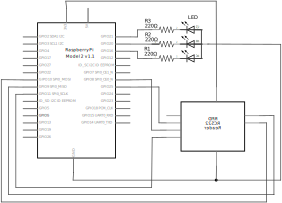
\includegraphics[width=0.9\textwidth]{../diagrams/reader_rfid_diagram_schem.png}	
	\caption{Schéma čtečky RFID}
	\label{fig:reader_rfid_diagram_schem}
\end{figure}

\subsection{Instalace}

Návod na instalaci sytému \texttt{Raspbian Jessie} naleznete na oficiálních stránkách: \\ \url{https://www.raspberrypi.org/documentation/installation/installing-images/README.md}
\\\\
\texttt{SSH protokol} je z důvodu bezpečnosti ve výchozím stavu zakázán. Návod pro povolení naleznete na stránce: \\ \url{https://www.raspberrypi.org/documentation/remote-access/ssh/}
\\\\
V konfiguraci \texttt{Raspberry Pi} povolte tyto položky:
\begin{itemize}[noitemsep]
\item [-] \texttt{Internationalisation Options} -> \texttt{SPI}
\item [-] \texttt{Advanced Options} -> \texttt{GPIO}
\end{itemize}
\ \\
Příkaz pro otevření konfigurace:
\begin{verbatim}
sudo raspi-config
\end{verbatim}
\ \\
\texttt{Python} je součástí \texttt{Raspbianu}, potřebné balíčky se budou instalovat z \texttt{Python Package Index (PyPI)}. K tomu slouží nástroj \texttt{pip}. Tento nástroj je standardně nainstalován v \texttt{Raspbian Jessie} (ale ne \texttt{Jessie Lite}). Můžete jej nainstalovat pomocí příkazu: 
\begin{verbatim}
sudo apt-get install python-pip
\end{verbatim}
\ \\
Následující příkaz nainstaluje všechny potřebné balíčky: 
\begin{verbatim}
sudo pip install -r requirements.txt
\end{verbatim}

\subsection{Spuštění}
Příklad spuštění s nastavením adresy serveru:

\begin{verbatim}
python ./reader_rfid/ -H 10.10.90.26
\end{verbatim}
\ \\
Volitelné parametry:
\begin{itemize}[noitemsep]
	\item \texttt{-h} ... vypíše nápovědu
	\item \texttt{-v} ... vypíše verzi
	\item \texttt{-d} ... zapne logování levelu debug
	\item \texttt{-H} ... adresa serveru
	\item \texttt{-p} ... port pro připojení k serveru
\end{itemize}


	\section{Mobilní aplikace}
	

Aplikace je určena pro \texttt{Android 6.0} a vyšší.	
Soubor \texttt{BPINI-1.4.2.apk} nahrajte do mobilního zařízení a spusťte instalaci.
Při instalaci bude potřeba dočasně povolit \texttt{instalaci z neznámých zdrojů}.
Po dokončení najdete aplikaci v menu mezi ostatními aplikacemi.


\chapter{Uživatelský manuál}

	\section{Čtečka RFID}
Čtečka svůj stav signalizuje pomocí LED diody, její stavy viz \ref{table:led_states}.

\begin{table}[ht]
\centering
\begin{tabular}{ c | p{6cm} }
\textbf{LED dioda} & \textbf{Popis} \\ \hline\hline
vypnuta & není navázáno připojení \\ \hline  
svítí zelená & režim přidávání položek \\ \hline
svítí červeně & režim odebírání položek \\ \hline
bliká zeleně & akce proběhla úspěšně \\ \hline
bliká červeně & nastala nečekaná chyba  \\ \hline
bliká modře & tag nemá nastavenou žádnou funkci  \\ \hline
\end{tabular}
\caption{Stavy LED diody}
\label{table:led_states}
\end{table}
\ \\
Tag načtený čtečkou se automaticky zaeviduje. Funkčnost tagu potom můžeme nastavit v mobilní aplikaci.
Je-li čtečka v režimu přidávání položek a načte-li tag reprezentující položku, přičte se k položce +1 množství.
K přepínání režimů slouží speciální tag typu "režim".



	\section{Mobilní aplikace}
	
\subsection{Přihlášení}	
	
Při prvním spuštění aplikace se zobrazí přihlašovací formulář viz \ref{fig:Screenshot_20170610-134211}.
Zadejte adresu serveru, pak následuje uživatelské jméno a heslo. 
\\\\
Výchozí přihlašovací údaje administrátora systému jsou:
\begin{itemize}[noitemsep]
\item [-] uživatelské jméno: admin
\item [-] heslo: heslo
\end{itemize}
\ \\	
\begin{figure}[h]
	\centering
	\includegraphics[width=0.3\textwidth]{../images/client_android/Screenshot_20170610-134211.png}	
	\caption{Přihlašovací formulář}
	\label{fig:Screenshot_20170610-134211}
\end{figure}

\newpage
\subsection{Menu}
Menu se zobrazí stisknutím hamburger menu nebo vysunutím z poza okraje viz \ref{fig:Screenshot_20170607-164924}.
První položka menu otevírá detail přihlášeného uživatele.
Na  řádce jsou výše zmíněné "Položky", pak následují "Tagy".
Další položkou v menu je "Čtečka", ta je dostupná jen pro mobilní zařízení s \texttt{NFC}, ostatním se nezobrazí.
Poté následují "Zařízení" a "Uživatelé", které jsou přístupné jen pro administrátora.
Poslední je "O aplikaci", zobrazí verzi, popis a autora aplikace.

\begin{figure}[h]
	\centering
	\includegraphics[width=0.3\textwidth]{../images/client_android/Screenshot_20170607-164924.png}	
	\caption{Menu aplikace}
	\label{fig:Screenshot_20170607-164924}
\end{figure}


\subsection{Položky}	

Po spuštění aplikace se zobrazí seznam položek skladu viz \ref{fig:Screenshot_20170607-164919}.
Položky můžete přidat pomocí zeleného plus v pravém dolním rohu a kliknutím na danou položku editovat.
Položku lze smazat jen tehdy, když se její počet rovná nule.

\begin{figure}[h]
	\centering
	\includegraphics[width=0.3\textwidth]{../images/client_android/Screenshot_20170607-164919.png}	
	\caption{Položky skladu}
	\label{fig:Screenshot_20170607-164919}
\end{figure}

\subsection{Tagy}

Tagy nelze přidávat ručně, jen pomocí čtečky. Kliknutím na tag se zobrazí editace, která nabízí změnu typu. Tag může být tří typů:
\begin{description}
\item [neznámý] - tag nemá nastavenou žádnou funkci
\item [režim] - tag umožňuje čtečce RFID přepínat režimy přidat/odebrat položku
\item [položka] - tag reprezentuje položku ve skladu 
\end{description}
\ \\

\begin{figure}[h]
	\centering
	\includegraphics[width=0.3\textwidth]{../images/client_android/Screenshot_20170607-164958.png}	
	\caption{Tagy}
	\label{fig:Screenshot_20170607-164958}
\end{figure}
\subsection{Čtečka}
Čtečka čekající na přiložení tagu viz \ref{fig:Screenshot_20170607-165058}.
Po přiložení tagu se načtou detailní informace viz \ref{fig:Screenshot_20170607-165117}, ale pokud není v systému zaevidován, pak je vytvořen tag typu "neznámý".


\begin{figure}
	\centering
  \begin{subfigure}[b]{0.3\textwidth}
    \centering
	\includegraphics[width=\textwidth]{../images/client_android/Screenshot_20170607-165058.png}	
	\caption{Připravená čtečka}
	\label{fig:Screenshot_20170607-165058}
  \end{subfigure}
  %
  \begin{subfigure}[b]{0.3\textwidth}
    \centering
	\includegraphics[width=\textwidth]{../images/client_android/Screenshot_20170607-165117.png}	
	\caption{Načtený tag}
	\label{fig:Screenshot_20170607-165117}
  \end{subfigure}
  \caption{Čtečka}
\end{figure}

\subsection{Administrace}

Seznam zařízení se ukazuje jen administrátorům viz \ref{fig:Screenshot_20170607-165221}. Zařízení se evidují automaticky při jakémkoli pokusu o připojení k serveru. Aby se zařízení připojilo, je nutné, aby konkrétnímu zařízení byl povolen přístup. Ten se mění pomocí přepínače.

\begin{figure}[h]
	\centering
	\includegraphics[width=0.3\textwidth]{../images/client_android/Screenshot_20170607-165221.png}	
	\caption{Zařízení}
	\label{fig:Screenshot_20170607-165221}
\end{figure}
\ \\
Jen administrátor má přístup ke správě uživatelů viz \ref{fig:Screenshot_20170607-165248}.
Dostat se na vytvoření nového uživatele je možné přes zelené plus v pravém dolním rohu a kliknutím na uživatele editovat.
Uživatele s rolí "administrátor" může vytvářet a editovat jen výchozí administrátor.

\begin{figure}[h]
	\centering
	\includegraphics[width=0.3\textwidth]{../images/client_android/Screenshot_20170607-165248.png}	
	\caption{Uživatelé}
	\label{fig:Screenshot_20170607-165248}
\end{figure}


	
	

\chapter{Obsah přiloženého CD}


\end{document}